\documentclass{article}
\usepackage{amsmath, amssymb, mdwlist, graphicx, hyperref}
\usepackage{listings,color}
\usepackage{wrapfig}
\usepackage[usenames,dvipsnames]{xcolor}
\definecolor{gray}{rgb}{0.97,0.97,0.97}
\lstset{%
language=C,%
%backgroundcolor=\color{gray},
emph={putpixel},
emphstyle=\bf,
tabsize=4,
framesep=5pt,
mathescape=true,
xleftmargin=0.1cm,
xrightmargin=0.1cm,
frame=lines,
%basicstyle=\ttfamily,
%keywordstyle=\color{Blue},
%commentstyle=\color{OliveGreen},
%stringstyle=\color{MidnightBlue},
columns=flexible,
%showstringspaces=false
}

\newcommand{\mpar}[1]{\marginpar{\textit{#1}}}
\newcommand{\norm}[1]{\Vert #1 \Vert}
\DeclareMathOperator{\argmax}{argmax}
\DeclareMathOperator{\argmin}{argmin}
\newenvironment{solution}{\paragraph{Solution.}$\,$ }{\vskip 3mm\hrule}
\newenvironment{exercise}[2]{\paragraph{Exercise #1 (#2pt).} }{
\medskip}
\newcommand{\bbR}{\mathbb{R}}
\newcommand{\bw}{\mathbf{w}}
\newcommand{\bx}{\mathbf{x}}
\newcommand{\bd}{\mathbf{d}}
\newcommand{\bb}{\mathbf{b}}
\newcommand{\by}{\mathbf{y}}
\newcommand{\bzero}{\mathbf{0}}
\newcommand{\bz}{\mathbf{z}}
\newcommand{\bSigma}{\mathbf{\Sigma}}
\newcommand{\bp}{\mathbf{p}}
\newcommand{\bP}{\mathbf{P}}
\newcommand{\bm}{\mathbf{m}}
\newcommand{\bc}{\mathbf{c}}
\newcommand{\bM}{\mathbf{M}}
\newcommand{\bV}{\mathbf{V}}
\newcommand{\bK}{\mathbf{K}}
\newcommand{\bD}{\mathbf{D}}
\newcommand{\bA}{\mathbf{A}}
\newcommand{\bX}{\mathbf{X}}
\newcommand{\bY}{\mathbf{Y}}
\newcommand{\bR}{\mathbf{R}}
\newcommand{\bI}{\mathbf{I}}
\newcommand{\bS}{\mathbf{S}}
\newcommand{\bT}{\mathbf{T}}
\newcommand{\balpha}{\boldsymbol{\alpha}}
\newcommand{\pt}[2]{\left(\begin{array}{c}#1\\#2\end{array}\right)}

\begin{document}
\title{MTAT.03.015 Computer Graphics (Fall 2013)\\
Exercise session XI: Raytracing.}
\author{Konstantin Tretyakov, Ilya Kuzovkin}
\date{November 18, 2013}
\maketitle

In this exercise session we shall study the basics of raycasting, raytracing and raymarching. For simplicity and convenience we shall be using the ShaderToy website\footnote{\url{https://www.shadertoy.com/}} and implement our raytracing code as a fragment shader\footnote{Note, that although GLSL's fragment shaders are conceptually very well suited for implementing raytracing-based techniques, in practice you would not be able to use them for large scenes. Firstly, there is a limit to the amount of data you can keep within the shader code. Secondly, GLSL lacks dynamic memory structures and recursion, which makes it impossible or hard to implement several algorithms. Finally, efficient raytracing may require multiple passes over the whole image -- something not possible within a single fragment shader.}.

The solutions will have to be submitted as a set of text files, zipped in a single archive. Solution to exercise $N$ should be saved in a file named \texttt{exercise}$N$\texttt{.glsl}.

\section{Basic Raycasting}
Let us start with a basic raycasting example. The idea of raycasting is to send rays from the eye through each pixel on screen and check for each ray, whether it intersects any geometry in the scene. The two main steps of a raycasting algorithm are therefore the following:
\paragraph{1. Convert pixel coordinates to a ray direction.}
It is best understood using the following diagram:
\begin{center}
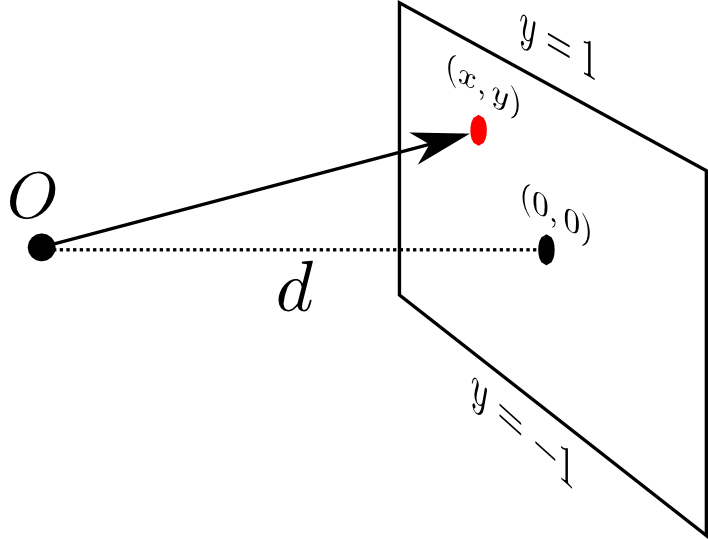
\includegraphics[width=0.4\textwidth]{fig1.png}
\end{center}
Assume our screen is positioned at distance $d$ from the origin. Let the center of the screen have pixel coordinates $(0, 0)$, the top and bottom correspond to $y=1$ and $y=-1$ respectively. If we assume that the camera is looking along the negative $z$ direction, the direction of the ray passing through pixel $(x,y)$ is $(x, y, -d)$. The parameter $d$ is related to the field of view angle $\alpha_y$:
$$\frac{1}{d} = \tan\left(\frac{\alpha_y}{2}\right).
$$

\paragraph{2. Cast the ray and look for intersections with objects in the scene.} Given the ray origin point $O$ (which corresponds to the camera position, i.e. $(0, 0, 0)$ in our case) and the ray direction that we computed in the previous step, we can check for each primitive in the scene whether it is intersected by the ray, and return the color of the pixel at the closest intersection point.

\begin{exercise}{1}{0.5}
The code base for this exercise is provided on the ShaderToy website at \url{https://www.shadertoy.com/view/ldSGzW}. Examine the code. We would like to raycast the following scene:
\begin{center}
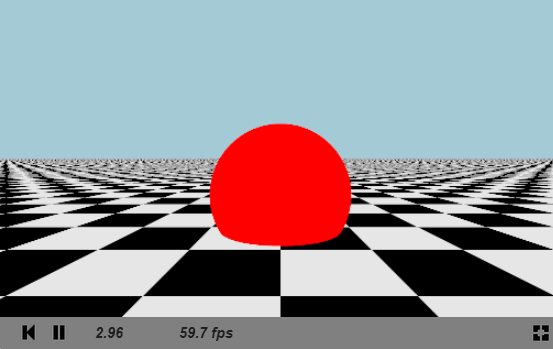
\includegraphics[width=0.7\textwidth]{raycasting.png}
\end{center}
The scene consists of a red sphere and a plane with a checkerboard pattern. The code base provides the specifications for both the plane and the sphere in the variables \texttt{plane} and \texttt{sphere}. The colors of the sky and the sphere are provided in the \verb#sky_color# and \verb#sphere_color# variables. The color of the plane is given as a function: \verb#plane_color# takes a point on the plane and returns its color.

The methods for finding ray-object intersection are also given to you: functions \verb#raycast_plane# and \verb#raycast_sphere# return the distance from ray origin to the intersection with the corresponding object, or \verb#INFINITY# if the ray does not hit the object. Your task is to introduce three changes to the code:
\begin{enumerate}
\item First implement the function \verb#raycast_scene#. The function should return the color of the object that is hit by the given ray first.
\item Next, change the main function so that the resulting image would have a $y$ field of view of 60 degrees.
\item At this point you will see the scene rendered like on the picture above. However, it will have a lot of aliasing artifacts: the sphere has jagged edges and the checkerboard pattern turns into nonsense at a distance. Let us fix this using a simple 3x3 discrete box filter. That is, rather than using a single ray for pixel $(x,y)$, cast 9 rays, as if you would be rendering pixels $\{x-0.2, x, x+0.2\}\times\{y-0.2, y, y+0.2\}$, and average the results\footnote{You are free to try larger grids, however note that having long nested loops in shader code may lead to weird results on some graphics cards. Also note that the use of \texttt{break} statement in \texttt{for}-loops can sometimes result in strange behaviour.}. 
\end{enumerate}
\end{exercise}

\section{Raytracing}
Let us now extend the basic raycasting algorithm we just implemented to support shadows and reflections. This results in what is typically referred to as \emph{recursive raytracing}. Open the code base given at \url{https://www.shadertoy.com/view/Ms2GzW}. This is a slightly extended version of the previous exercise. Note the following changes:
\begin{enumerate}
\item \textbf{Lighting.}  We shall now be using lighting computations. Consequently, rather than specifying object colors, we specify their materials in \verb#sphere_mat# and \verb#plane_mat()#. Ambient light is given in the \verb#ambient# variable, and a single light source is described in \verb#light#.
Finally, the function \verb#lighting# implements the familiar Blinn-Phong light model. Note that this function takes a \verb#viewer_pos# argument rather than assuming the viewer to be fixed at $(0, 0, 0)$. Think why it is done this way.
\item \textbf{More detailed raycasting.} The \verb#raycast_scene# routine is updated to not only return the distance to the closest object, but also the actual point location, the normal at that point and the material of the object.
\item The actual scene rendering routine, \verb#render_scene# is separate from the raycasting function (which is now just a useful primitive).
\end{enumerate}

\begin{exercise}{2}{1}
Update the function \verb#render_scene# to implement recursive raytracing with shadows and reflections.
\begin{enumerate}
\item To implement shadows, cast a ray from the point towards the light source. If this \emph{shadow ray} hits anything on the way, you can consider the point to be in shadow (and thus only affected by ambient light).
\item To implement reflections, note that the \verb#Material# structure has a field \verb#reflectivity#. This is the weight with which the reflected ray contributes to the visible color of a point with this material. The full color of a point is then its ``usual'' color + reflectivity weight times the color ``seen'' by the reflected ray. Implement at least two reflection steps. (Hint: this is naturally done using a loop).
\end{enumerate}
The resulting image should look as follows:
\begin{center}
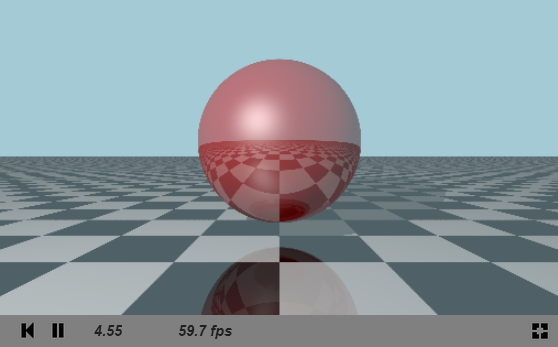
\includegraphics[width=0.7\textwidth]{raytracing.png}
\end{center}

Hint: Remember that ray direction vectors must always be normalized.

Hint: You can use the \texttt{reflect} GLSL function to compute reflection vectors.
\end{exercise}

\begin{exercise}{3*}{0.5}
An example of a great purely-raytracing based scene is the shader ``Relentless'': \url{https://www.shadertoy.com/view/lss3WS}. Study the code. Your task is to add a perfectly reflective sphere right in front of the camera, getting a result like the following:
\begin{center}
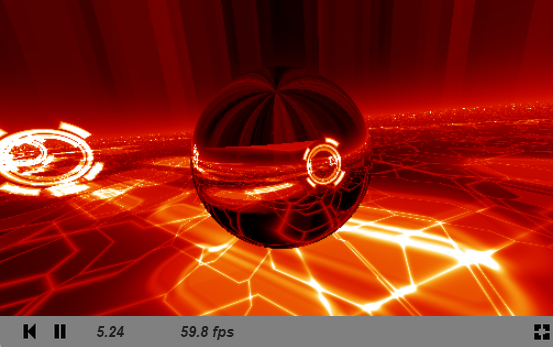
\includegraphics[width=0.7\textwidth]{relentless.png}
\end{center}
Let the sphere radius be $1$. Have its center positioned straight in front of the camera, at distance $2$. For simplicity you may assume that the sphere is always the topmost object (i.e. resolve ray intersection with the sphere first of all, ignoring the possibility of other objects being in front).
\end{exercise}

\section{Raymarching}
When objects have complex descriptions, it may be easier to search for ray-object intersections using iterative numerical methods, resulting in the family of \emph{raymarching} algorithms. \emph{Sphere tracing} is a particularly fast version of raymarching, which can be applied if the scene is modeled as a \emph{distance field}. A distance field is a function that for any point $(x, y, z)$ returns the distance to the nearest object in the scene. For example, if the scene consists of a single sphere of radius R centered at the origin, the corresponding distance function is as simple as
$$
f(\bp) = \Vert \bp \Vert - R
$$

Distance fields are a very flexible means for modeling complex scenes, see \url{http://www.iquilezles.org/www/articles/distfunctions/distfunctions.htm}.
%The normal to a point on a surface described by a distance field can be obtained by simply taking the normalized gradient of the field at that point:
%$$
%\text{normal}(\bp) \propto \nabla f(\bp) \approx \frac{1}{\varepsilon}\left(f(\bp+(\varepsilon, 0, 0)), f(\bp+(0, \varepsilon, 0)), f(\bp+(0, 0, \varepsilon))\right).
%$$

\begin{exercise}{4}{0.5}
Open the code in \url{https://www.shadertoy.com/view/MsjGRD}. The \texttt{main} function presents you with a familiar structure of a raytracer. The only difference is that all the hard work is done by a function named \texttt{raymarch} now rather than \texttt{raycast}. Implementing this function is your first task. 

The function \texttt{raymarch(ro, rd)} must ``walk'' from the point \texttt{ro} in the direction \texttt{rd}, making steps of size \texttt{scene(x)}, looking for a point \texttt{x} where the function \texttt{scene} becomes nearly zero. If you implement this algorithm correctly, you should see the rendering of the scene, which is a simple rounded box:
\begin{center}
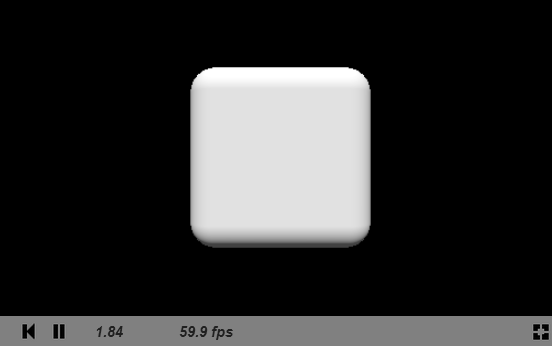
\includegraphics[width=0.7\textwidth]{raymarching1.png}
\end{center}
\end{exercise}


\begin{exercise}{5}{0.5}
Next, let us make the scene a bit more interesting. For that we shall use some of the basic operations with distance field functions, that are already given to you in the code. Make the changes to the \texttt{scene} function, so that instead of a static rounded box, the scene would become a rotating grid of rounded boxes, each with a hole drilled in it. That is, turn the scene into this:
\begin{center}
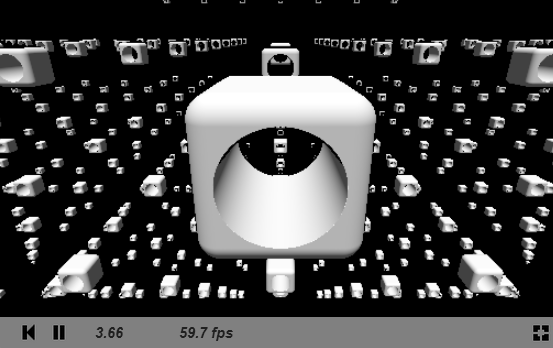
\includegraphics[width=0.7\textwidth]{raymarching2.png}
\end{center}
The comments in the code will provide you the appropriate parameter values.
\end{exercise}

\begin{exercise}{6*}{0.5}
Modify the code so that the insides of the holes, drilled in the cubes would be colored red:
\begin{center}
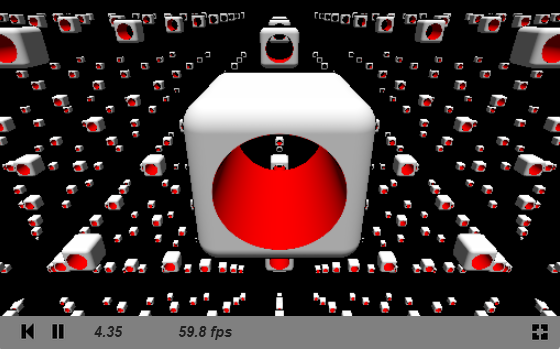
\includegraphics[width=0.7\textwidth]{raymarching3.png}
\end{center}
Hint: For this you will need to change the \texttt{scene} function so that it would not only return the distance, but also the color of the corresponding region of the field. The simplest approach is to have \texttt{scene} return a \texttt{vec4} (instead of a \texttt{float}), so that its first three components correspond to the color and the fourth is the distance.
\end{exercise}

\begin{exercise}{7*}{0.5}
Add reflections to the raymarching algorithm:
\begin{center}
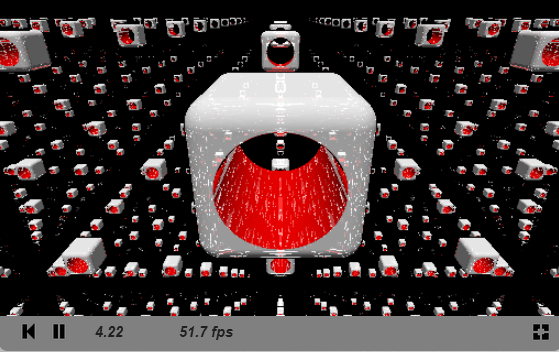
\includegraphics[width=0.7\textwidth]{raymarching4.png}
\end{center}
Hint: The approach is similar to the one used in Exercise 2. Make a new function \texttt{render}, that will invoke \texttt{raymarch} inside a loop, accumulating the resulting color as a weighted sum of multiple reflections. Assume the reflectivity coefficient to be $0.2$.
\end{exercise}


\begin{exercise}{8*}{1}
Read the article \emph{Distance Estimated 3D Fractals}\footnote{\url{http://blog.hvidtfeldts.net/index.php/2011/06/distance-estimated-3d-fractals-part-i/}}. Present a shader implementation of any Mandelbulb fractal.
\end{exercise}

\end{document}
